\chapter{The Sun in the Sky: Days and Seasons}\label{ch:g3:sun-days-seasons}

In June you play outside after dinner in golden \omterm{def:g1:light-and-shadows:source}{light}; in December
the streetlamps come on before you are home from school. The Sun
keeps its old habit --- up one side, over the top, down the other ---
but its road through the sky is not the same road all year. Follow
it for a whole year, and you discover the \omterm{def:g3:sun-days-seasons:year}{seasons}.

\section{The Sun's changing road}

\begin{example}[Summer road, winter road]\label{ex:g3:sun-days-seasons:roads}
Watch the Sun's arc in midsummer: it rises early, climbs very high
--- almost overhead at midday --- and sets late: a long, high road,
and a long day. In midwinter, the arc is low and short: the Sun
rises late, never climbs far above the rooftops, and sets in the
middle of the afternoon. Between the two, in spring and autumn, the
road is middling --- and day and night share the \omterm{ex:g2:measuring-time:clock}{hours} almost
equally.
\end{example}

\begin{omfigure}
\begin{tikzpicture}[scale=0.85]
  \draw[thick] (0,0) -- (11,0);
  \draw[dashed, omThm, thick] (1.0,0.2) .. controls (3.5,4.6)
    and (7.5,4.6) .. (10.0,0.2);
  \fill[omThm] (5.5,3.5) circle (0.3);
  \node[above, font=\small, omThm] at (5.5,3.9) {midsummer: high and long};
  \draw[dashed, omDef, thick] (2.6,0.15) .. controls (4.4,1.7)
    and (6.6,1.7) .. (8.4,0.15);
  \fill[omDef] (5.5,1.3) circle (0.3);
  \node[above, font=\small, omDef] at (2.9,1.35) {midwinter: low and short};
\end{tikzpicture}

{\small The Sun's two extreme roads over the same horizon. The high
summer arc takes many \omterm{ex:g2:measuring-time:clock}{hours} to travel; the low winter arc is done by
mid-afternoon.}
\end{omfigure}

\begin{proposition}[The midday rule]\label{prop:g3:sun-days-seasons:midday}
In every \omterm{def:g3:sun-days-seasons:year}{season}, the Sun stands highest in the middle of the day ---
and at that moment every \omterm{def:g1:light-and-shadows:shadow}{shadow} is at its shortest for the day and
points in the same direction as yesterday's midday \omterm{def:g1:light-and-shadows:shadow}{shadow}, and
tomorrow's. Midday \omterm{def:g1:light-and-shadows:shadow}{shadows} are the most reliable arrows in nature.
\end{proposition}

\begin{example}[Reading the season from a shadow]\label{ex:g3:sun-days-seasons:shadowlength}
The \emph{length} of the midday \omterm{def:g1:light-and-shadows:shadow}{shadow} changes with the \omterm{def:g3:sun-days-seasons:year}{season}: in
summer, with the Sun nearly overhead, the midday \omterm{def:g1:light-and-shadows:shadow}{shadow} of a post is
a short stump; in winter, with the Sun hanging low, the same post
throws a long midday \omterm{def:g1:light-and-shadows:shadow}{shadow}. Mark the tip of the midday \omterm{def:g1:light-and-shadows:shadow}{shadow} on
the ground once a month, and the marks will crawl back and forth
through the year like a slow pendulum.
\end{example}

\section{The shadow clock}

\begin{definition}[Sundial]\label{def:g3:sun-days-seasons:sundial}
A \emph{sundial}\index{sundial} is a clock made of a \omterm{def:g1:light-and-shadows:shadow}{shadow}: a stick
or blade standing in the sun, with marks around it showing where the
\omterm{def:g1:light-and-shadows:shadow}{shadow} falls at each hour. As the Sun travels its arc, the \omterm{def:g1:light-and-shadows:shadow}{shadow}
sweeps around the marks --- slowly, silently, and without a single
moving part.
\end{definition}

\begin{method}[Building a shadow clock]\label{met:g3:sun-days-seasons:build}
On a sunny morning, in a spot that stays sunny all day:
\begin{enumerate}
  \item plant a straight stick upright in flat ground (or stand it
        in a bucket of sand);
  \item every hour, on the hour, mark the tip of its \omterm{def:g1:light-and-shadows:shadow}{shadow} with a
        pebble and write the hour on the pebble with chalk;
  \item keep going until evening.
\end{enumerate}
Tomorrow, the \omterm{def:g1:light-and-shadows:shadow}{shadow} will visit your pebbles on schedule: your stick
now tells the time. (For a while, at least --- as the \omterm{def:g3:sun-days-seasons:year}{season} slides,
the \omterm{def:g1:light-and-shadows:shadow}{shadows} slide too, and your pebbles will slowly drift wrong.)
\end{method}

\begin{omfigure}
\begin{tikzpicture}[scale=0.85]
  \draw[thick] (0.5,0) -- (10.5,0);
  \draw[very thick] (5.5,0) -- (5.5,1.7);
  \draw[line width=3pt, omExo] (5.5,0) -- (2.2,0.9);
  \draw[line width=3pt, omExo, opacity=0.6] (5.5,0) -- (4.1,1.35);
  \draw[line width=3pt, omExo, opacity=0.35] (5.5,0) -- (5.5,1.5);
  \draw[line width=3pt, omExo, opacity=0.6] (5.5,0) -- (6.9,1.35);
  \draw[line width=3pt, omExo] (5.5,0) -- (8.8,0.9);
  \node[font=\footnotesize] at (1.8,1.0) {morning};
  \node[font=\footnotesize] at (5.5,1.9) {midday: shortest};
  \node[font=\footnotesize] at (9.4,1.0) {evening};
\end{tikzpicture}

{\small One stick, one day: the \omterm{def:g1:light-and-shadows:shadow}{shadow} sweeps like a slow hand,
longest at the day's edges, shortest at midday.}
\end{omfigure}

\section{The year and its seasons}

\begin{definition}[The year and the seasons]\label{def:g3:sun-days-seasons:year}
While the Earth spins once a day, it also travels along a huge
journey \emph{around the Sun} --- one full lap takes a
\emph{year}\index{year}, about $365$ days. Along the lap, the Sun's
road through our sky slowly rises and falls, and we pass through the
four \emph{seasons}\index{season}: spring, summer, autumn, winter
--- then spring again, lap after lap.
\end{definition}

\begin{example}[The four quarters]\label{ex:g3:sun-days-seasons:quarters}
Summer: high Sun, long days, short midday \omterm{def:g1:light-and-shadows:shadow}{shadows}. Winter: low Sun,
short days, long midday \omterm{def:g1:light-and-shadows:shadow}{shadows}. Spring and autumn sit between ---
and in each of them comes one special day when daytime and night
last equally long. Farmers, sailors and builders of old learned to
read this calendar straight from the sky.
\end{example}

\begin{omfigure}
\begin{tikzpicture}[scale=0.85]
  \fill[omThm] (5.5,1.8) circle (0.5);
  \foreach \a in {0,30,...,330} {
    \draw[omThm] (5.5,1.8) ++(\a:0.68) -- ++(\a:0.26);
  }
  \draw[dashed, thick] (5.5,1.8) ellipse (4.4 and 1.55);
  \fill[omDef] (1.1,1.8) circle (0.26);
  \fill[omDef] (9.9,1.8) circle (0.26);
  \fill[omDef] (5.5,3.35) circle (0.26);
  \fill[omDef] (5.5,0.25) circle (0.26);
  \node[left, font=\small] at (0.75,1.8) {winter here};
  \node[right, font=\small] at (10.25,1.8) {summer here};
  \node[above, font=\small] at (5.5,3.7) {spring};
  \node[below, font=\small] at (5.5,-0.1) {autumn};
\end{tikzpicture}

{\small One lap of the Earth around the Sun --- one year, four
\omterm{def:g3:sun-days-seasons:year}{seasons}. Why the low road in winter and the high road in summer?
That secret is kept for a later chapter on the Sun--Earth--Moon
family.}
\end{omfigure}

\begin{remark}[Winter is not ``farther'']\label{rem:g3:sun-days-seasons:notfarther}
It is tempting to guess that winter is cold because the Earth drifts
farther from the Sun. Not so --- the distance barely changes, and
when it is winter here, it is summer for children on the far half of
the Earth at the very same moment, which no ``farther away'' could
explain! The real key is the Sun's \emph{low road}: low Sun, slanted
\omterm{def:g1:light-and-shadows:source}{light}, weak warming. The full explanation is promised for a later
chapter.
\end{remark}

\begin{omfigure}
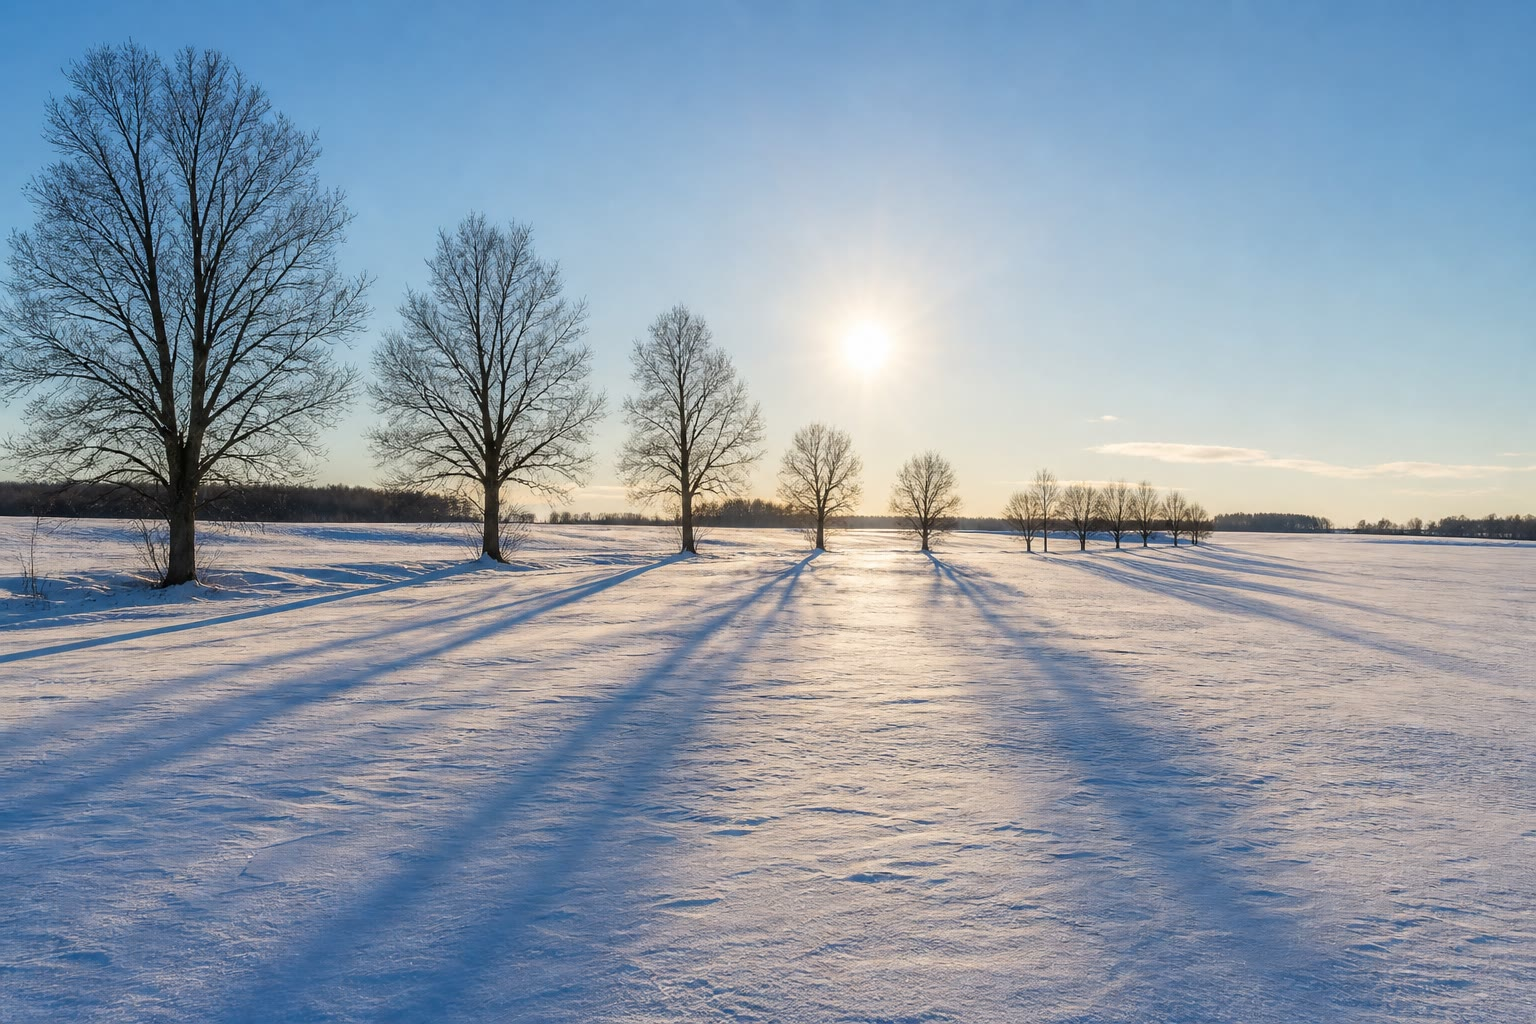
\includegraphics[width=0.58\linewidth]{images/book1/ai/g3-seasons-winter-sun.jpg}

{\small A winter midday: the Sun stays low, the \omterm{def:g1:light-and-shadows:source}{light} comes in slanting, and the \omterm{def:g1:light-and-shadows:shadow}{shadows} run long across the snow.}
\end{omfigure}

\section{Exercises}

\begin{exercise}[$\star$]\label{exo:g3:sun-days-seasons:1}
In which \omterm{def:g3:sun-days-seasons:year}{season} is the Sun's arc highest and longest? Lowest and
shortest? What does that do to the length of the day?
\end{exercise}

\begin{exercise}[$\star$]\label{exo:g3:sun-days-seasons:2}
At what moment of the day is a post's \omterm{def:g1:light-and-shadows:shadow}{shadow} shortest? What else is
special about the midday \omterm{def:g1:light-and-shadows:shadow}{shadow}, day after day?
\end{exercise}

\begin{exercise}[$\star$]\label{exo:g3:sun-days-seasons:3}
The same post throws a midday \omterm{def:g1:light-and-shadows:shadow}{shadow} of $2$ boots' length in June
and $7$ boots in December. Explain the difference with the Sun's
two roads.
\end{exercise}

\begin{exercise}[$\star$]\label{exo:g3:sun-days-seasons:4}
How does a \omterm{def:g3:sun-days-seasons:sundial}{sundial} tell the time? What is its moving hand made of?
\end{exercise}

\begin{exercise}[$\star$]\label{exo:g3:sun-days-seasons:5}
In \cref{met:g3:sun-days-seasons:build}, why must the stick stay in
a spot that is sunny all day? What happens to the clock in cloudy
weather --- and at night?
\end{exercise}

\begin{exercise}[$\star$]\label{exo:g3:sun-days-seasons:6}
How long does the Earth take for one lap around the Sun? How many
\omterm{def:g3:sun-days-seasons:year}{seasons} fit in one lap? Put them in order, starting from spring.
\end{exercise}

\begin{exercise}[$\star$]\label{exo:g3:sun-days-seasons:7}
About how many days are in a year? And --- from an earlier chapter
--- how many \omterm{ex:g2:measuring-time:clock}{hours} in a day? Which journey of the Earth makes each?
\end{exercise}

\begin{exercise}[$\star$]\label{exo:g3:sun-days-seasons:8}
Name two clues, visible from your window in a single week, that
tell you whether you are in midsummer or midwinter without a
calendar.
\end{exercise}

\begin{exercise}[$\star$]\label{exo:g3:sun-days-seasons:9}
When it is winter where you live, what \omterm{def:g3:sun-days-seasons:year}{season} is it for children on
the far half of the Earth? What does this prove about the guess
``winter happens because the whole Earth is farther from the Sun''?
\end{exercise}

\begin{exercise}[$\star\star$]\label{exo:g3:sun-days-seasons:10}
A gardener plants her shadow-clock pebbles in March. In June the
\omterm{def:g1:light-and-shadows:shadow}{shadow} no longer touches the pebbles at the marked \omterm{ex:g2:measuring-time:clock}{hours}. Has the
stick moved? Explain what drifted, using
\cref{ex:g3:sun-days-seasons:shadowlength}.
\end{exercise}

\begin{exercise}[$\star\star$]\label{exo:g3:sun-days-seasons:11}
An explorer wakes with no watch and no phone, sees the Sun exactly
at its highest, and an hour later finds her tent's \omterm{def:g1:light-and-shadows:shadow}{shadow} already
longer than the tent is tall. Roughly what time was it when she
woke, and is she closer to midsummer or midwinter? Argue from the
midday rule and the \omterm{def:g1:light-and-shadows:shadow}{shadow}'s length.
\end{exercise}
